\documentclass{article}
\usepackage[margin=1in]{geometry}
\usepackage{amsmath,amsthm,amssymb}
\usepackage{bbm,enumerate,mathtools}
\usepackage{tikz,pgfplots}
\usepackage{chessboard}
\usepackage[hidelinks]{hyperref}
\usepackage{multicol} % Problem 35
\usepackage{xstring} % Difficulty command
\usetikzlibrary{shapes.geometric}

\newenvironment{question}{\begin{trivlist}\item[\textbf{Question.}]}{\end{trivlist}}
\newenvironment{note}{\begin{trivlist}\item[\textbf{Note.}]}{\end{trivlist}}
\newenvironment{references}{\begin{trivlist}\item[\textbf{References.}]}{\end{trivlist}}
\newenvironment{related}{\begin{trivlist}\item[\textbf{Related.}]\end{trivlist}\begin{enumerate}}{\end{enumerate}}

\newcommand\score[1]{
\pgfmathsetmacro\pgfxa{#1+1}
\tikzstyle{scorestars}=[
  star,
  star points=5,
  star point ratio=2.25,
  draw,
  inner sep=3pt,
  anchor=outer point 5
]
  \begin{tikzpicture}[baseline]
    \draw[opacity=0] (0,-0.5) rectangle (0,0.2); % Workaround for whitespace at the bottom.
    \foreach \i in {1,...,4} {
      \pgfmathparse{(\i<=#1?"yellow":"gray")}
      \edef\starcolor{\pgfmathresult}
      \draw (\i*4.5ex,0) node[name=star\i,scorestars,fill=\starcolor]  {};
    }
  \end{tikzpicture}
}

\newcommand{\difficulty}[1]{%
  \IfEqCase{#1}{%
      {1}{
        
\begin{tikzpicture}[scale=0.7, baseline=0.9mm]%
          \definecolor{slopegreen}{rgb}{0.0, 0.5, 0.0}%
          \fill[slopegreen] (0.5,0.5) circle (0.5);%
        \end{tikzpicture}%
      }%
      {2}{
        
\begin{tikzpicture}[scale=0.7, baseline=0.9mm]%
          \definecolor{slopeblue}{rgb}{0.0, 0.44, 1.00}
          \fill[slopeblue] (0,0) rectangle (1,1);%
        \end{tikzpicture}%
      }%
      {3}{
\begin{tikzpicture}[scale=0.7, baseline=0.9mm]\fill (0,0.5)--(0.5, 0)--(1,0.5)--(0.5,1)--cycle; \end{tikzpicture}}%
      {4}{
\begin{tikzpicture}[scale=0.7, baseline=0.9mm]\fill (0.25,0)--(0,0.5)--(0.25,1)--(0.5,0.5)--cycle; \fill (0.75,0)--(0.5,0.5)--(0.75,1)--(1,0.5)--cycle;\end{tikzpicture}}%
      % you can add more cases here as desired
  }[\PackageError{difficulty}{Undefined difficulty level: #1}{}]%
}%
\newcommand{\rating}[2]{\difficulty{#1}\\\score{#2}\\}


\begin{document}
\rating{2}{3}
Let $G$ be a finite group, and call a sequence $\{g_i \in G\}_{i=1}^{|G|-1}$ a
\textit{Hamiltonian walk} if for each $g \in G$ there exists some $i \geq 0$
such that the $n$-th partial product $p_n = g$ where
$p_n = g_1 \cdot g_2 \cdots g_n$.
\begin{figure}[ht!]
  \centering
  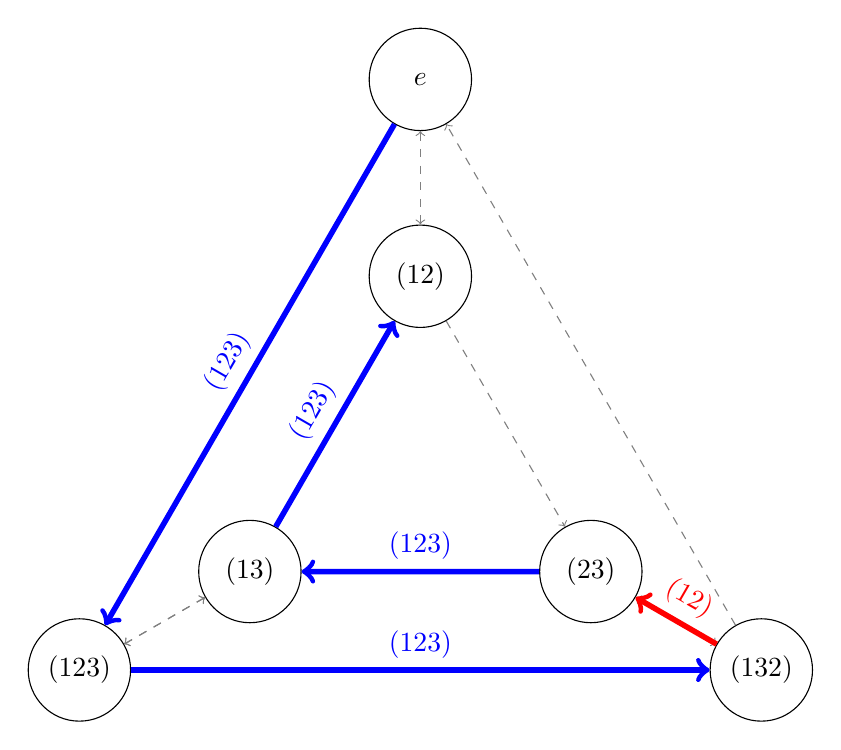
\begin{tikzpicture}[scale=2.5]
    \node[draw, circle, minimum size = 1.3cm] (e)   at (0,2)               {$e$};
    \node[draw, circle, minimum size = 1.3cm] (12)  at (0,1)               {$(12)$};
    \node[draw, circle, minimum size = 1.3cm] (123) at ({-sqrt(3)},-1)     {$(123)$};
    \node[draw, circle, minimum size = 1.3cm] (13)  at ({-sqrt(3)/2},-1/2) {$(13)$};
    \node[draw, circle, minimum size = 1.3cm] (132) at ({sqrt(3)},-1)      {$(132)$};
    \node[draw, circle, minimum size = 1.3cm] (23)  at ({sqrt(3)/2},-1/2)  {$(23)$};

    % \foreach \v in {e,12,123,13,132,23} {
    %   \foreach \w in {e,12,123,13,132,23} {
    %     \draw [thin, gray] (\v) to (\w);
    %   }
    % }
    \draw [thin, gray, dashed, <->] (e) to (12);
    \draw [thin, gray, dashed, <->] (23) to (132);
    \draw [thin, gray, dashed, <->] (13) to (123);
    \draw [thin, gray, dashed, <->] (13) to (123);
    \draw [thin, gray, dashed, ->] (12) to (23);
    \draw [thin, gray, dashed, ->] (132) to (e);
    \draw[->, line width = 0.2em, blue] (e) to node[sloped,above]{$(123)$} (123);
    \draw[->, line width = 0.2em, blue] (123) to node[sloped,above]{$(123)$} (132);
    \draw[->, line width = 0.2em, red] (132) to node[sloped,above]{$(12)$} (23);
    \draw[->, line width = 0.2em, blue] (23) to node[sloped,above]{$(123)$} (13);
    \draw[->, line width = 0.2em, blue] (13) to node[sloped,above]{$(123)$} (12);
  \end{tikzpicture}
  % \begin{alignat*}{2}
  %   p_0 & = e, &&\\
  %   p_1 &= (123), &&\\
  %   p_2 &= (123)(123) &&= (132),\\
  %   p_3 &= (132)(12)  &&= (23),\\
  %   p_4 &= (23)(123) &&= (13),\ \text{and}\\
  %   p_5 &= (13)(132) &&= (12).
  % \end{alignat*}
  \caption{
    An example showing that the sequence $((123),(123),(12),(123),(123))$
    is a palindromic Hamiltonian walk for $S_3$, where
    $p_0 = e$,
    $p_1 = (123)$,
    $p_2 = (132)$,
    $p_3 = (23)$,
    $p_4 = (13)$, and
    $p_5 = (12)$.
  }
\end{figure}

\begin{question}
  Does every finite group have a Hamiltonian walk that is a palindrome?
\end{question}

\begin{related}
  \item If not, does every finite group have a Hamiltonian walk whose reversal is
    also a Hamiltonian walk?
  \item Is there an efficient way to compute how many
    \textit{essentially different} Hamiltonian walks $G$ has?
  \item For a group $G$, what proportion of Hamiltonian walks are reversible?
  \item Does every finite semigroup have a reversible Hamiltonian walk?
\end{related}

\begin{references}
  \item Problem 79.
  \item \url{https://math.stackexchange.com/q/3706654/121988}
\end{references}
\end{document}
